\documentclass[../thesis/thesis.tex]{subfiles}
\renewcommand{\baselinestretch}{1.5}\selectfont
\graphicspath{{../figs/ch2-rfmwmeas/}}

\begin{document}
%\begin{refsection}
\setcounter{chapter}{1}
\chapter{Radio Frequency and Microwave \\Measurements}
\section{Introduction}

To characterise nonlinear behavioural models, the radio frequency (RF) response of a device to electromagnetic wave stimuli must be measured. When compared with DC (and low frequency) measurements, RF and microwave measurements present significant additional challenges. 
For DC systems, it is desirable to propagate voltages through a circuit with minimal loss in amplitude. To achieve this effectively, components are typically designed with high input impedance and low output impedance. With RF systems, circuit components and interconnects can be of the order of a quarter-wavelength in length, and therefore signals must be treated as electromagnetic waves to account for different behaviour at these frequencies.
When a travelling wave encounters a discontinuity in impedance, such as a cable connector or on-wafer structure, some of the power in the wave is reflected. The amount of reflected power is proportional to the size of the impedance mismatch between each side of the discontinuity. Hence, for most RF systems, the transmission of power is the focus of the circuit designer. The measurement of power flowing through a transmission line is complicated by three key factors. Firstly, because the waves are travelling, the instantaneous voltage at any point on the transmission line will vary between the peak-to-peak values of the wave. Secondly, waves travel in both directions along the transmission line and must be measured separately. Finally, the power of the wave is a complex quantity consisting of both magnitude and phase.
To perform these measurements, a specialist instrument called a vector network analyser (VNA) can be used. In this chapter, the concepts and measurements associated with this instrument are introduced, which will be used later in the thesis to understand the uncertainty contributions from measurements to nonlinear behavioural models.

\section{Electromagnetic Wave Parameters}
\subsection{Wave Definitions}

To describe the power of electromagnetic waves propagated through a transmission line, several definitions are in use in industry and academia for either accuracy or convenience. To avoid confusion in this document, these will now be defined. Information presented in this section has been obtained from \cite{Williams_2013,Marcuvitz_1951,Marks_1992,Kurokawa_1965,Williams_2001}.

\subsubsection{Travelling Waves}

Travelling waves represent a solution to Maxwell's equations along a transmission line. They are physical and measurable via slotted line experiments or ``thru-reflect-line'' calibrations (explained later in this Chapter). Travelling waves are defined by the total transverse electric and magnetic fields $\bm{E}_\textrm{t}$ and $\bm{H}_\textrm{t}$ of a single propagating mode at each frequency:
\begin{equation}
\bm{E}_\textrm{t}=c^+e^{-\gamma z}\bm{e}_\textrm{t}+c^-e^{+\gamma z}\bm{e}_\textrm{t},\quad
\bm{H}_\textrm{t}=c^+e^{-\gamma z}\bm{h}_\textrm{t}-c^-e^{+\gamma z}\bm{h}_\textrm{t}
\end{equation}
where, following the notation of \cite{Williams_2001}, $\bm{e}_\textrm{t}$ and $\bm{h}_\textrm{t}$ are the un-normalized electric and magnetic fields of the modal solution of Maxwell’s equations in transmission line, $\gamma=a+ib$ is the complex propagation constant of the mode, $z$ is the direction of propagation, and $c^+$ and $c^-$ are complex quantities representing the un-normalized forward and backward amplitude of the mode, respectively.

\subsubsection{Equivalent-Circuit Voltage and Current}

To represent travelling waves as equivalent low frequency circuit parameters such as voltage and current, a normalisation is chosen to derive a characteristic impedance for the transmission line. This normalisation takes the form:
\begin{equation}
\bm{E}_\textrm{t}(z)=\dfrac{v(z)}{v_0}\bm{e}_\textrm{t},\quad
\bm{H}_\textrm{t}(z)=\dfrac{i(z)}{i_0}\bm{h}_\textrm{t},
\end{equation}
where $v_0$ and $i_0$ are normalisation constants that allow $v$ and $i$ to take units of root-mean-square voltage and current, respectively \cite{Williams_2001}.

\subsubsection{Pseudowaves}

Equivalent voltages and currents cannot be used in lossy transmission lines where the electric and magnetic fields are out of phase. To account for this and provide a solution which can be used with conventional circuit design methodologies (e.g. Smith chart techniques \cite{Smith_1939}) and simulators, pseudowaves can be used. This representation is defined with a reference impedance, $Z_\textrm{ref}$, which can be chosen by the user, but is typically 50-$\Omega$ in conventional measurements. The forward and backward pseudowaves $a$ and $b$ can be written as:
\begin{equation}
a(Z_\textrm{ref})=\bigg[\dfrac{|v_0|}{v_0}\dfrac{\sqrt{\Re(Z_\textrm{ref})}}{2|Z_\textrm{ref}|}\bigg](v+iZ_\textrm{ref}),\quad b(Z_\textrm{ref})=\bigg[\dfrac{|v_0|}{v_0}\dfrac{\sqrt{\Re(Z_\textrm{ref})}}{2|Z_\textrm{ref}|}\bigg](v-iZ_\textrm{ref})
\end{equation}

\subsubsection{Power Waves}

Finally, power waves are defined so that the relationship $P = |a|^2 - |b|^2$ is true for any reference impedance, where $P$ is the power transmitted through the transmission line and $a$ and $b$ are the forward and backward power waves, respectively. They are defined as:
\begin{equation}
a(Z_\textrm{ref})=\dfrac{v+iZ}{2\sqrt{\Re(Z_\textrm{ref})}},\quad b(Z_\textrm{ref})=\dfrac{v-iZ^*}{2\sqrt{\Re(Z_\textrm{ref})}}.
\end{equation}
Data taken from Keysight instruments used later in this work is presented in power wave format, with units of square-root Watts. To convert these values into decibels referenced to 1 milliwatt, the following formula is used:
\begin{equation}
P(\textrm{dBm}) = 10\log_{10}(P(\sqrt{W})^2) + 30
\end{equation}

\subsection{Derived Metrics and Figures of Merit}

The behaviour of a linear microwave device can be completely defined by the complex ratio of electromagnetic waves which are scattered at each port to those which are incident at each port. The combination of these ratios constitutes the scattering parameters (S-parameters) of a microwave device and are used extensively in the design and measurement of microwave systems \cite{Pozar_2004}. The formal definitions of the S-parameters for a two-port device are:
\begin{equation}
S_{11}=\dfrac{b_1}{a_1}\bigg\rvert_{a_2=0},\quad
S_{12}=\dfrac{b_1}{a_2}\bigg\rvert_{a_1=0},\quad
S_{21}=\dfrac{b_2}{a_1}\bigg\rvert_{a_2=0},\quad
S_{22}=\dfrac{b_2}{a_2}\bigg\rvert_{a_1=0},
\label{ch2_eqn_sp}
\end{equation}
where both a and b can be expressed in either pseudowave or power wave representation. The term “scattered” can be interchanged with “transmitted” and “reflected” depending on if the scattered wave is output on a different port, or the same port, to the incident wave, respectively. A signal flow diagram is provided in Figure \ref{ch2_fig_filter} showing the relationship between equivalent-circuit voltage and current, pseudowaves/power waves and S-parameters for a two-port device.
The S-parameters of all microwave devices will exhibit some degree of frequency dependence. This effect originates from physical processes occurring in the device and can either be a benefit or hindrance to a design. Most passive components (including cables) will have a usable bandwidth which is an unwanted limitation, whereas microwave filters are a ubiquitous component where the same fixed bandwidth is the main purpose of the device. To capture this frequency dependence, S-parameters are measured across a frequency range and stored in a table, usually in Touchstone format (see Figure \ref{ch2_fig_s2p}). An example of the frequency dependence of a filter is shown in Figure \ref{ch2_fig_filter}. For a device operating in the linear regime, if multiple stimuli at different frequencies are incident on the device, they will not interact with each other. The scattered waves will have the same frequency components as if the stimulus at each frequency was applied separately. This is called the frequency superposition principle and does not apply to nonlinear operating regimes, which will be discussed later in this chapter.

\begin{figure}
	\centering
	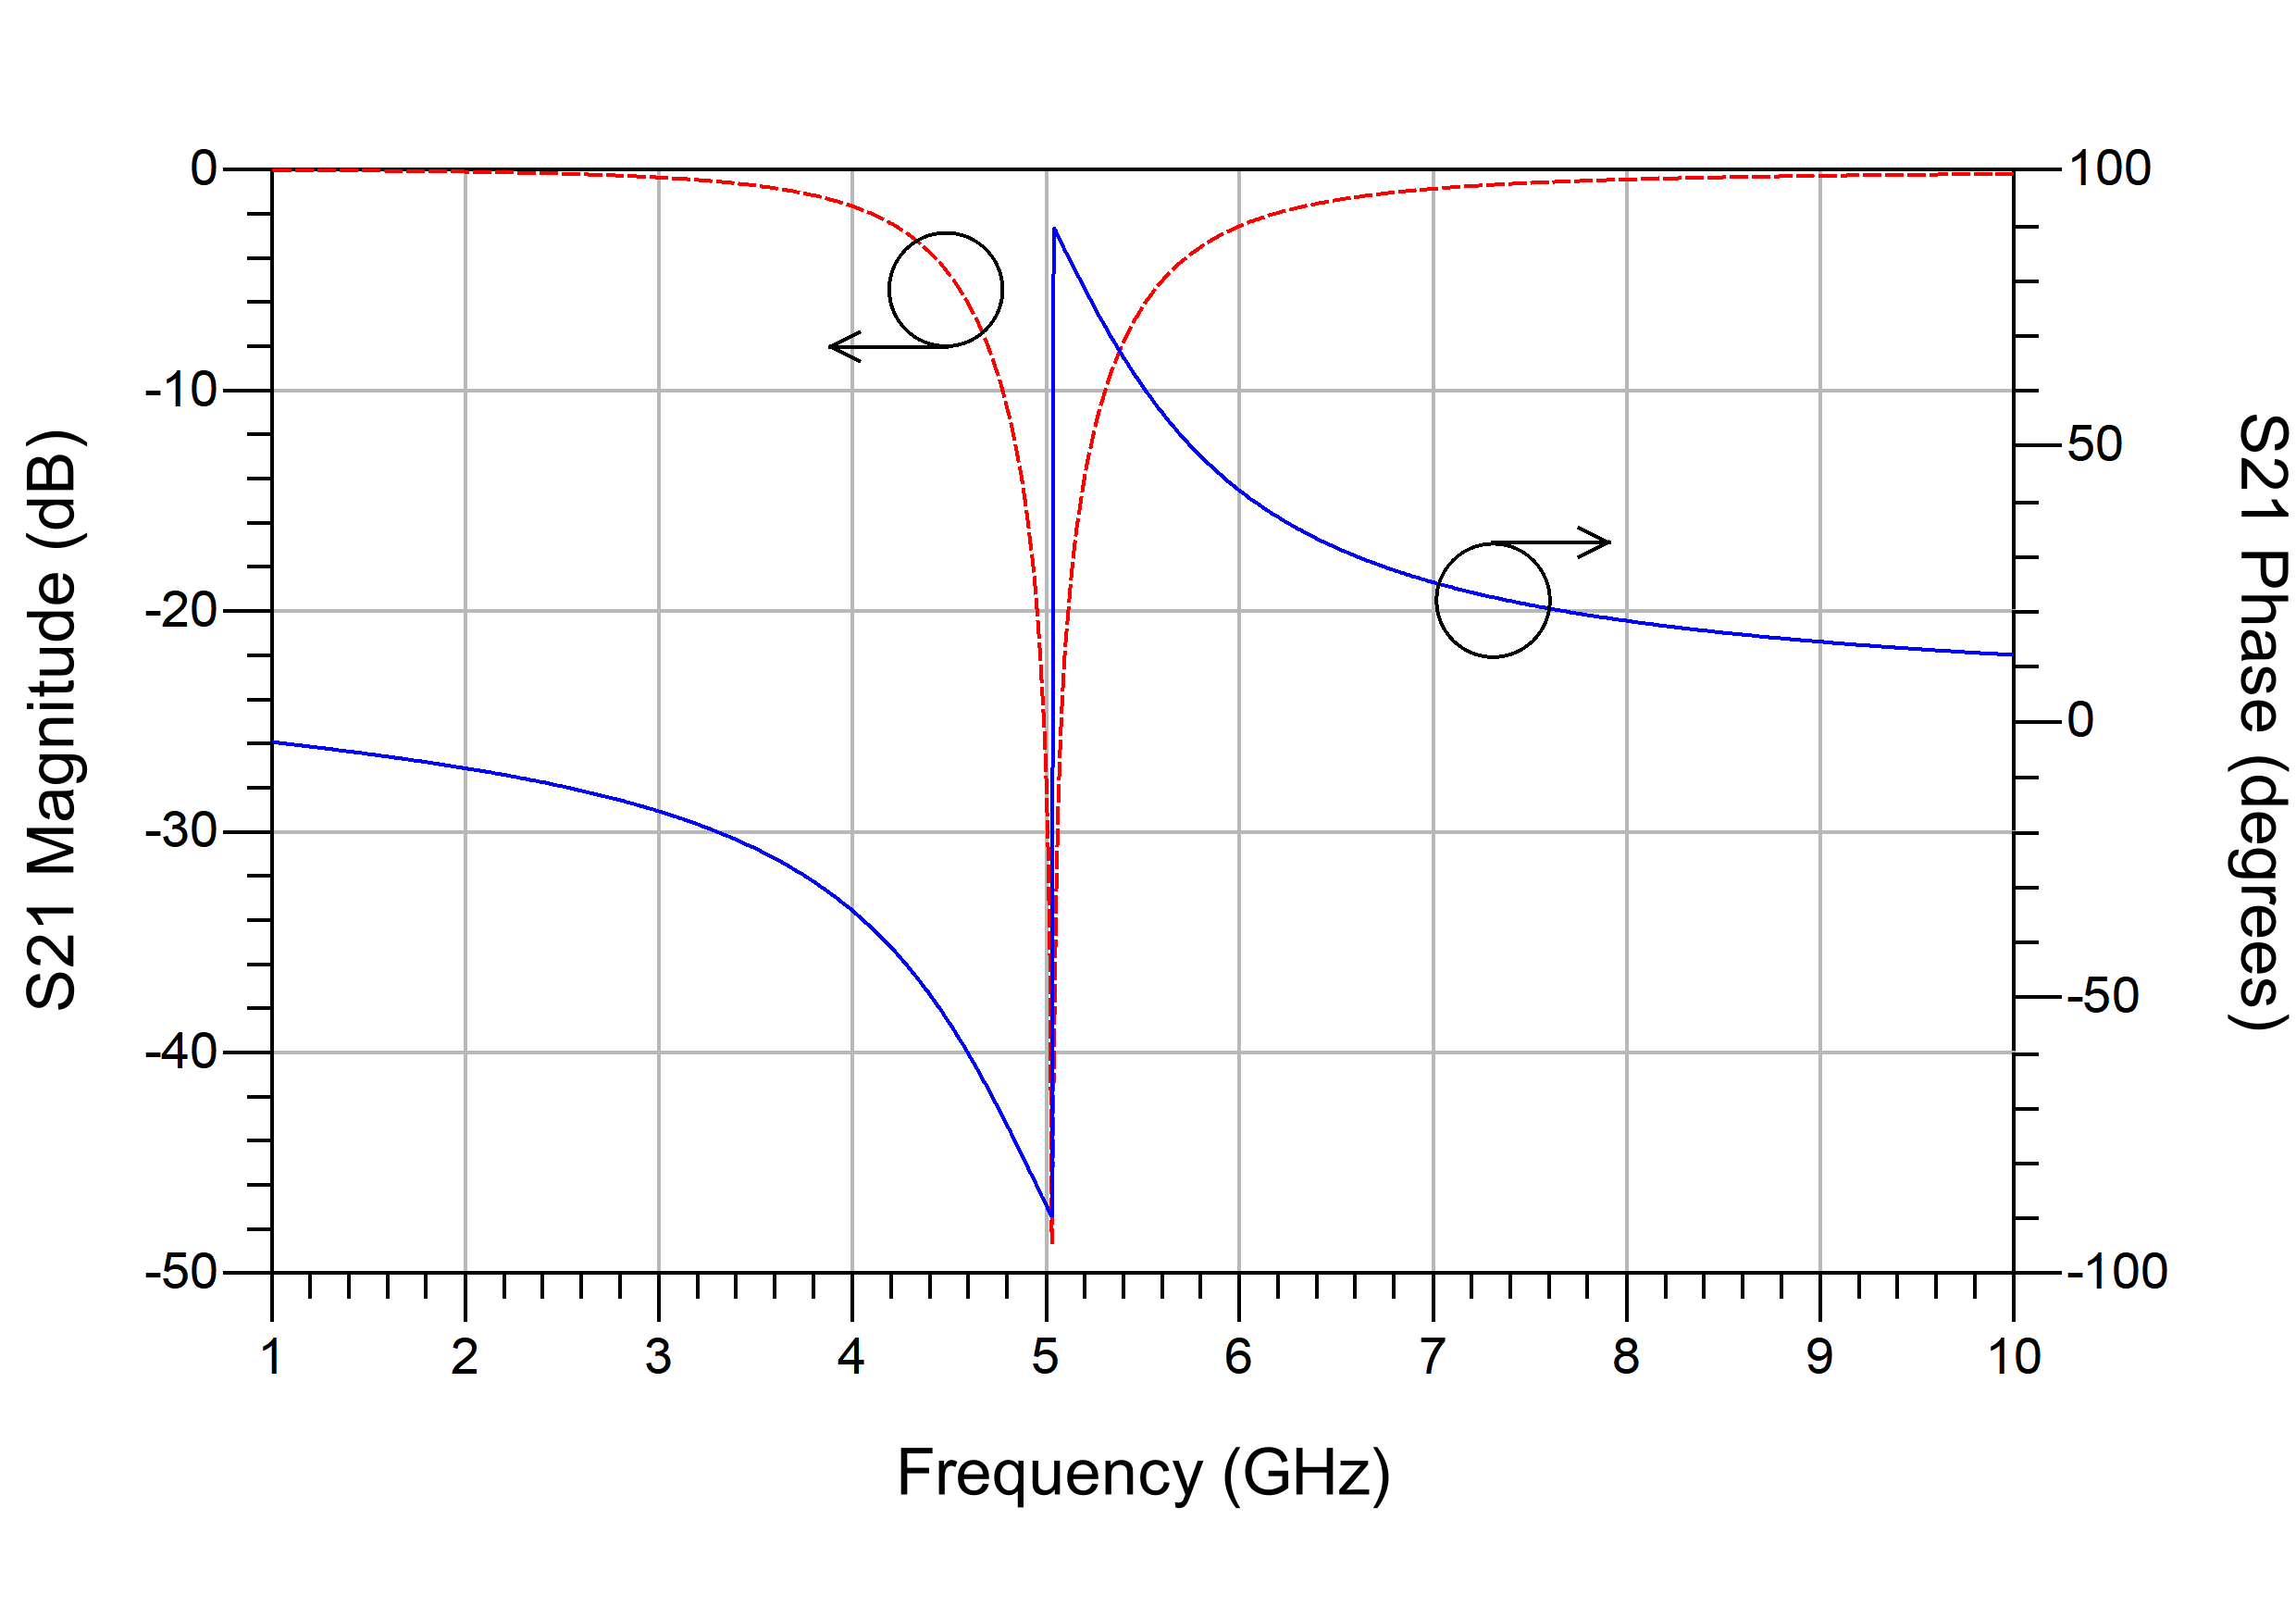
\includegraphics[width=0.8\textwidth]{ch2_filter}
	\caption[The frequency dependence of a bandstop filter.]{The frequency dependence of the magnitude (red dotted trace) and phase (blue solid trace) of $S_{21}$ for a bandstop filter.}
	\label{ch2_fig_filter}
\end{figure}

\begin{figure}
	\centering
	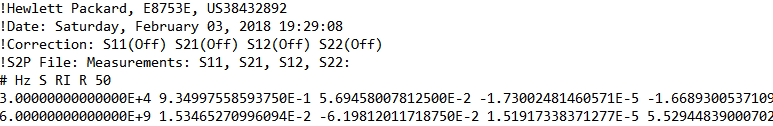
\includegraphics[width=\textwidth]{ch2_s2p}
	\caption[The Touchstone file layout.]{An short example Touchstone file showing a two-port measurement at two frequencies. The rows continue to the right of the figure.}
	\label{ch2_fig_s2p}
\end{figure}

Scattering parameters are often expressed in matrix form, where the column index is the scattered port, and the row index is the incident port. For a two-port device, the S-parameter matrix would be:
\begin{equation}
S=
\begin{bmatrix}
S_{11} & S_{12} \\
S_{21} & S_{22}
\end{bmatrix}
\end{equation}

The most useful characteristic of a two-port microwave device is often the effect which it has on a transmitted wave in the forward direction ($S_{21}$). If the device increases the magnitude of the incident signal this metric is called gain, otherwise it is called insertion loss. Typically gain is associated with active devices (those which are powered from an external source separate to the incident microwave signals) such as amplifiers, and insertion loss is associated with passive devices (those with no external power source) such as attenuators, splitters and mixers. The power gain (operating gain) and insertion loss relating to $S_{21}$ can be calculated using:
\begin{equation}
\textrm{Power Gain} = 10 \log_{10} |S_{21}|^2 \textrm{ dB},
\end{equation}
and:
\begin{equation}
\textrm{Insertion Loss} = -10 \log_{10} |S_{21}|^2 \textrm{ dB},
\end{equation}
respectively.

Optimal transmission in microwave systems requires impedance matching between components, and it is inevitable that this matching will not be perfect and so some power will be reflected in a two-port device. Therefore, the match of a device is another important measurement, which is dependent on the voltage reflection coefficient ($\Gamma$) of the device and can be related to the impedance of a source and load by:
\begin{equation}
\Gamma_{xx} = S_{xx} = \dfrac{Z_\textrm{L}-Z_\textrm{S}}{Z_\textrm{L}+Z_\textrm{S}},
\label{gamma1}
\end{equation}
where $x$ is a port index.
A more thorough definition of voltage reflection coefficient for a two-port device includes any effect from the impedance seen at the other port, and for the case of input match is calculated as:
\begin{equation}
\Gamma_{11} = S_{11} + \dfrac{S_{12}S_{21}\Gamma_\textrm{L}}
{1-S_{22}\Gamma_\textrm{L}},
\label{gamma2}
\end{equation}
where $\Gamma_\textrm{L}$ is the voltage reflection coefficient of the load connected to the device. For amplifiers, the amount of isolation (reduction of $S_{12}$) is an important characteristic of the device, whereby a fully isolated amplifier ($S_{12}=0$) is said to be unilateral and equations \ref{gamma1} and \ref{gamma2} are equivalent.

For active devices, such as amplifiers, it can also be useful to consider the power reflected at the input when calculating the power gain of the device. The transducer gain of a device accounts for this potential loss of power at the input and provides a more portable metric which is not dependent on the impedance of the measurement setup. It is defined as:
\begin{equation}
G_\textrm{T} = \dfrac{1-|\Gamma_\textrm{S}|^2}
{1-|\Gamma_\textrm{in}\Gamma_\textrm{S}|^2}
|S_{21}|^2
\dfrac{1-|\Gamma_\textrm{L}^2|^2}
{1-|S_{22}\Gamma_\textrm{L}|^2},
\end{equation}
where $\Gamma_\textrm{in}$ is the input match of the device.

For all devices operating in the linear regime, any reflected or transmitted wave will have a frequency equivalent to that incident to the device. In addition, the stimulus power that was used to measure the S-parameters is not important as the ratio of scattered to incident wave magnitude is not dependent on this quantity. However, when microwave devices operate in the nonlinear regime, these conditions no longer apply, and S-parameters cannot be used to capture the full behaviour of the device.

\section{Measurements of Nonlinear Devices}

Microwave devices operating in the nonlinear regime exhibit three differences from their linear counterparts which are significant to the designer.

Firstly, the amplitude of electromagnetic waves scattered from the device are not linearly dependent on the amplitude of waves incident. This is the cause of features such as gain compression and gain expansion in amplifiers. Some of these effects are solely due to the nonlinear sources inside the device, while others are a symptom of the combined response of the nonlinearity and the power supply. A typical gain compression curve is shown in Figure \ref{ch2_fig_comp}.

\begin{figure}
	\centering
	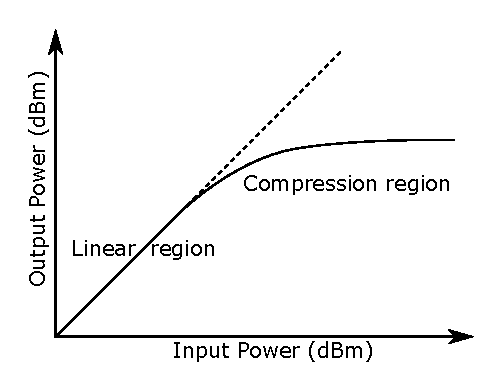
\includegraphics[width=0.5\textwidth]{ch2_compression}
	\caption[An illustration of gain compression.]{Gain compression occurs when an amplifier is driven into a nonlinear operating regime.}
	\label{ch2_fig_comp}
\end{figure}

Secondly, the frequency superposition principle does not apply, and instead the frequency spectrum of scattered waves contains components at frequencies other than those incident upon it. Rather than the incident signals purely summing inside the device, they are also multiplied with each other (frequency mixing), as shown by:
\begin{align}
b&=c_0+c_1a+c_2a^2+c_3a^3+\cdots,\\
\alpha=\beta&=2\pi\omega t,\\
a(t)&=A\cos(\alpha),\\
\cos(\alpha)\cos(\beta)&=\dfrac{1}{2}(\cos(\alpha+\beta)+cos(\alpha-\beta)),\\
a^2(t)&=\dfrac{1}{2}A^2[\cos(2\pi(2\omega)t)+1],\\
a^3(t)&=\dfrac{1}{4}A^3[\cos(2\pi(3\omega)t)+3\cos(2\pi\omega t)].
\end{align}
Here, $a$ and $b$ are the incident and scattered waves for the device, $c_i$ are coefficients of the device's nonlinear transfer function, and $a(t)$ is a wave in the time domain with amplitude $A$ and frequency $\omega$. For stimuli with a single frequency ($\alpha$=$\beta$, as above), integer multiples of that frequency will be scattered from the device (harmonics). For stimuli with multiple tones ($\alpha\ne\beta$), additional products from combinations of the incident tone frequencies will be scattered (intermodulation). If the nonlinear device is incident with a fixed bandwidth of frequencies, such as the case for communications signals, then sidebands will be produced around the harmonics of the oscillator frequencies. This effect can be troublesome in practical designs where the unwanted sidebands overlap with the useful microwave bandwidth, distorting the signal. For this reason, it is important for designers to be able to accurately measure and characterise this nonlinear effect. Figure \ref{ch2_fig_im3} shows example spectra of these effects.

\begin{figure}
	\centering
	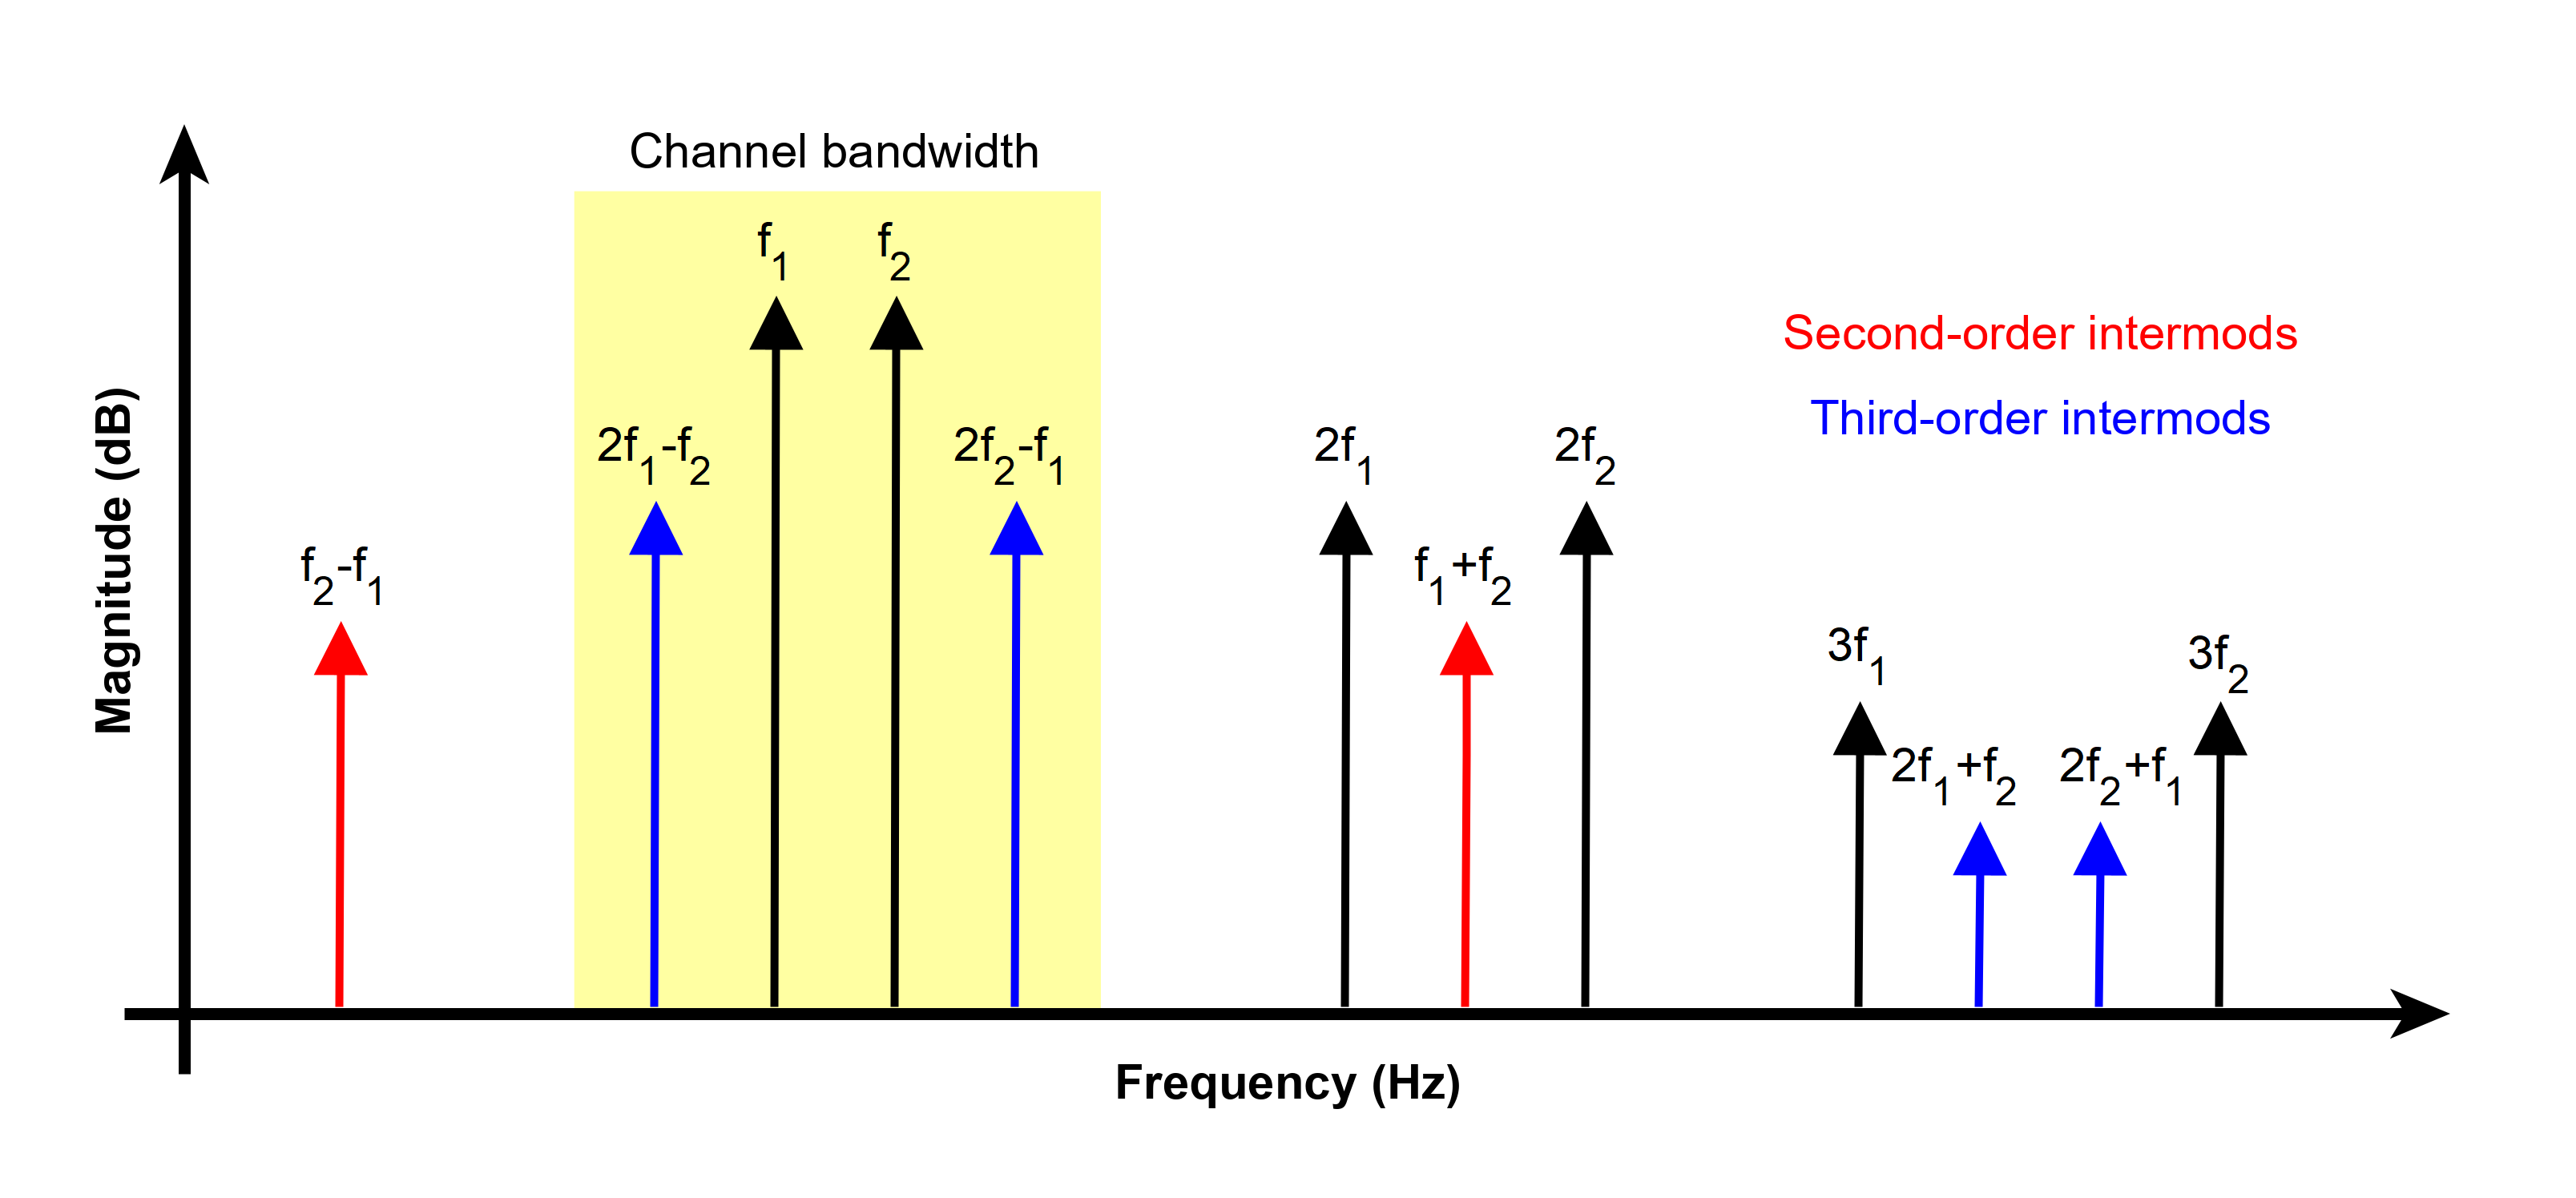
\includegraphics[width=\textwidth]{im3}
	\caption[Intermodulation products from two interacting tones.]{Intermodulation products from two tones within the cellular channel bandwidth $f_1$ and $f_2$. The second order products, and upper third order products, can be easily filtered out. However, the lower third order products $2f_1-f_2$ and $2f_2-f_1$ are located within the channel bandwidth and interact with the useful data, increasing error vector magnitude (EVM) and bit error rate (BER).}
	\label{ch2_fig_im3}
\end{figure}

Finally, the amplitude of scattered waves with multiple incident waves is dependent (nonlinearly) on the phase of incident waves. In the linear regime the superposition principle prevents this, but now there is a nonlinear dependence which can have significant effects on the amplitude of scattered waves. Designers must consider this when building efficient nonlinear amplifiers, which leads to the practice of accurately terminating scattered harmonic frequencies at an optimum phase. This will be covered in more detail in Chapter 5 when we discuss nonlinear device models. 

The result of these differences is that the measurement requirements for nonlinear devices are considerably larger than for linear devices. The nonlinear dependencies on stimulus power and phase means that ratioed measurements no longer fully capture the device response, and absolute measurements of the magnitude and phase of both the incident and scattered waves is required. The production of scattered waves at frequencies different to those in the stimulus demands an additional dimension of measurements. These complications must be met with changes to both the measurement system and the method of storing the results.

\section{Vector Network Analysers}

To measure the incident and scattered waves for a DUT and calculate the S-parameters as in (\ref{ch2_eqn_sp}), a vector network analyser (VNA) is typically used. The VNA is a quintessential piece of RF and microwave instrumentation and is found in most RF and microwave laboratories. Due to the challenging nature of measurements at these frequencies, it is a complicated instrument with many internal parts. This section explains how the VNA functions and the procedures behind its calibration. For a good history of VNA architecture and product development please refer to \cite{Teppati_2013,Dunsmore_2012,Rytting_2008}.

\subsection{Architecture}

The origin of the VNA lies in an early instrument called a reflectometer. Designed in 1947 by Parzen and Yalow \cite{Parzen_1947}, it became an invaluable tool for characterising transmission lines used in telecommunication systems. Shown in Figure \ref{ch2_fig_refl}, the incident signal is generated by a swept signal source and passes through the directional coupler before arriving at the DUT. The voltage reflection coefficient of the DUT will cause an amount of incident power to be reflected, which passes back through the coupler before being absorbed by the source (which has very low reflection). The directional couplers allow the waves travelling between the source and the DUT to be sampled by complex receivers, filtering the two waves by their direction of travel thus allowing the incident and scattered waves to be separated for measurement. 

\begin{figure}
	\centering
	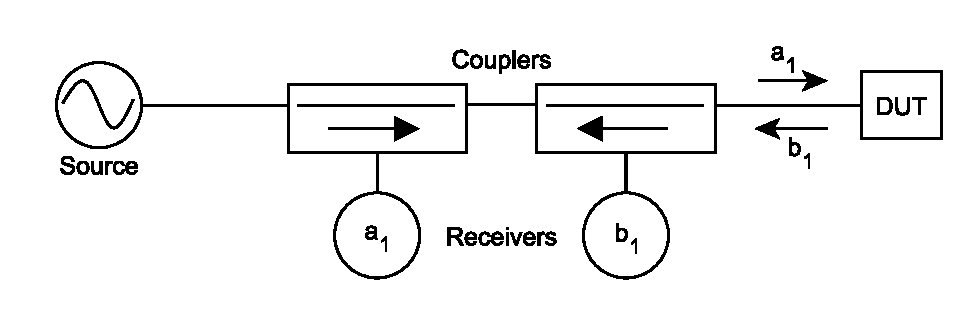
\includegraphics[width=0.8\textwidth]{ch2_reflect}
	\caption[Structure of a one-port reflectometer.]{A one-port simple reflectometer. $a_1$ is the incident wave generated by the source, which is admitted to the DUT while also being sampled by the directional coupler and sent to the reference receiver, R. The reflected wave, $b_1$, is also sampled by another directional coupler and sent to the test receiver, T, with the remaining power dissipated at the matched source.}
	\label{ch2_fig_refl}
\end{figure}

The limitation of a single reflectometer is that it can only measure waves at one port of a DUT, therefore preventing transmission measurements. By adding a second reflectometer and synchronising the stimuli and measurements, it is possible to measure all S-parameters of a two-port device. This is the fundamental structure of a VNA, and most variations consist of changing the number of sources or receivers to optimise the instrument for cost or performance. Many older designs use an economical single source which is switched between both ports, whereas now the price of sources has fallen, there are instruments available with two independent sources, which allows two-tone and some types of nonlinear measurements. These more versatile units often also expose more  connections between internal components (e.g. the couplers and receivers) to allow the user to perform non-standard measurements or to add attenuation or preamplification for higher stimulus powers.
Modern VNAs also offer the option of measuring more than two ports, which are referred to as “multi-port” measurements. Several manufacturers offer four-port instruments which include four reflectometers (with usually two sources), although with external switching networks it is possible to expand this up to 48 ports \cite{mj_multiport}.
The basic block diagram of a modern two-port double-reflectometer VNA is shown in Figure \ref{ch2_fig_vna}. To measure both stimulus conditions for the two-port S-parameter equations in (\ref{ch2_eqn_sp}), the sources alternate between delivering power and acting as a load for each measurement. As the source is swept the a and b waves for all ports are measured against frequency, from which the VNA software calculates the S-parameters. The receivers sampling the incident waves are known as the reference receivers and those sampling the scattered waves are called measurement or test receivers. The components in direct path between the source and the DUT (e.g. couplers) are historically called the test-set, which used to be interchangeable depending on the type of transmission line and test port connector family used.

\begin{figure}
	\centering
	
\includegraphics[width=0.6\textwidth]{ch2_vna}
	\caption[Structure of a two-source mixer-based VNA.]{A modern two-source mixer-based VNA, which employs heterodyning to allow measurements at microwave frequencies. Two directional couplers are located between each source and the DUT and are connected back to back. These sample waves travelling in both directions and are connected to mixers which downconvert the microwave frequencies (R) into intermediate frequencies (I) which can be sampled by the complex receivers. The shared local oscillator (LO) feeding the mixers preserves phase coherence between the receivers. This configuration is known as a two-port double-reflectometer VNA. Figure adapted by author from \cite{Root_2013}.}
	\label{ch2_fig_vna}
\end{figure}

To perform S-parameter measurements using a VNA, the user must set both the frequency span and number of frequency points. They may also change settings of intermediate frequency bandwidth (IFBW) and numerical averaging, both of which reduce measurement noise by applying digital filtering but can consequently increase acquisition time. The user will then perform a calibration, which corrects for any response present in the measurement setup that is not caused by the DUT. During calibration, physical ``measurement planes'' are defined at the closest interface to the DUT. All ``corrected'' measurements performed after the calibration will capture the s-parameter response between these planes, including any adapters or other components between them and the DUT. After calibration, it is good practice to check that it was successful by measuring some known devices (verification \cite{Collier_2007}), or to use techniques such as ripple extraction (discussed in Chapter 4) to measure the residual uncertainty. This process characterises any remaining error which the calibration failed to correct.

\subsection{Error Models}

The calibration process involves characterising an error model which represents the response of the test-set and any cables and adapters between the VNA and the DUT. These error models are stored in the memory of the VNA and are typically de-embedded from the raw measurements before the results are presented to the user (although the raw measurements can still be obtained for separate post-processing). Because the measurement setup response is frequency dependent, the error model coefficients are characterised across the measurement bandwidth and are either applied at each measurement frequency or linearly interpolated. A popular review of VNA error models is provided in \cite{Rytting_2000} but two particular models, used in the work presented in this dissertation, will now be described.

\subsubsection{One-Port Model}

\begin{figure}
	\centering
	
\includegraphics[width=\textwidth]{ch2_oneport}
	\caption[The three-term VNA error model.]{The three-term error model for a one-port measurement, which sits between the VNA receivers measuring $a_0$ and $b_0$ waves and the DUT with reflection coefficient $\Gamma$. The error box contains coefficients ($e_{00}, e_{10}, e_{01}, e_{11}$) which act like S-parameters, and captures unwanted effects from both the VNA internal components and and external test setup (e.g. cables and adapters).}
	\label{ch2_fig_oneport}
\end{figure}

The classic one-port error model can be obtained through analysis of the signal flow diagram of a one-port VNA shown in Figure \ref{ch2_fig_oneport}. One can write the relationship between the measured ($\Gamma_\textrm{m}$) and actual ($\Gamma$) reflection coefficients as:
\begin{equation}
\Gamma_\textrm{m}=\frac{b_0}{a_0}=\frac{e_{00}-(\overbrace{e_{00}e_{11}-e_{01}e_{10}}^\Delta)\Gamma}{1-e_{11}\Gamma},
\end{equation}
from which the actual reflection coefficient can be obtained using the measured value and three error coefficients using:
\begin{equation}
\Gamma=\frac{\Gamma_\textrm{m}-e_{00}}{e_{11}\Gamma_\textrm{m}-\Delta}.
\label{ch2_eqn_oneport1}
\end{equation}

The three coefficients relate to unwanted physical effects occurring between the VNA receivers and the DUT. Directivity ($e_{00}$) is caused by the nonideal operation of the directional couplers used to separate the incident and reflected waves inside the VNA. In practice, some amount of incident wave will travel into the test receiver port, reducing the measured gain of the device under test.
Test port match ($e_{11}$) results from the impedance of the VNA test port (either the original test port or the extended measurement plane including any cables or other components in the setup) being different from the characteristic impedance of the measurement, which is typically 50-$\Omega$. This effect will cause some of the incident wave to be reflected at the test port which is not due to the device response.
Reflection tracking ($\Delta$) characterises the insertion loss of the couplers and other measurement components between the reference receiver and the test receiver.

\subsubsection{Eight-Term Model}

Devices with two or more ports require transmission measurements in addition to the reflection measurements corrected using the one-port model. Historically, two-port VNAs used a single reference receiver and a test receiver for each channel. This meant that the reference receiver would be shared between ports one and two, requiring a separate error model for each configuration (``forward'' and ``reverse'') \cite{Rehnmark_1974}. This resulted in the 12-term and 10-term models which were the standard two-port VNA error models implemented in firmware. More recently, VNAs have employed dedicated reference receivers for each measurement port. Because the calibrated signal path (reference receiver to DUT) does not change when the stimulus is switched between ports one and two, a simpler error model can be used. This model is called the eight-term model (or error box model) and is illustrated in Figure \ref{ch2_fig_twoport}. The eight-term model also ignores error due to crosstalk between test ports, which is usually appropriate for coaxial and waveguide measurements but not for on-wafer measurements where the probes may couple. In this case the 16-term model provides greater accuracy \cite{Butler_1991}.

\begin{figure}
	\centering
	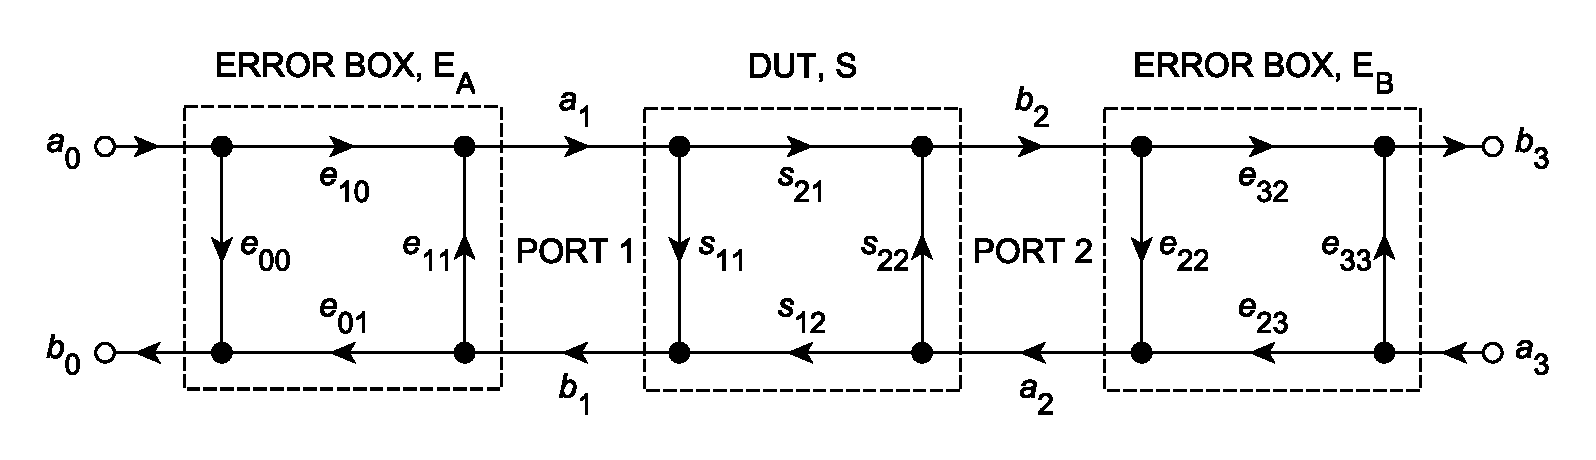
\includegraphics[width=\textwidth]{ch2_twoport}
	\caption[The eight-term VNA error model.]{The eight-term error model for a two-port measurement. Similar to the three-term model for one-port measurements, an S-parameter model is used capture the error coefficients between the Port 1 receivers ($a_0$, $b_0$) and the DUT ($e_{00}, e_{10}, e_{01}, e_{11}$), and a separate model used between the Port 2 receivers ($a_3$, $b_3$) and the DUT ($e_{22}, e_{32}, e_{23}, e_{33}$).}
	\label{ch2_fig_twoport}
\end{figure}

The model defines two error boxes, $\mathbf{E}_\textrm{A}$ and $\mathbf{E}_\textrm{B}$, associated with ports one and two, respectively:

\begin{align}
	\begin{bmatrix}
		b_0 \\
		a_1 \\
	\end{bmatrix}
	&=
	\underbrace{
		\begin{bmatrix}
			e^\textrm{A}_{00} & e^\textrm{A}_{01} \\
			e^\textrm{A}_{10} & e^\textrm{A}_{11} \\
		\end{bmatrix}
	}_{\mathbf{E}_\textrm{A}}
	\begin{bmatrix}
		a_0 \\
		b_1 \\
	\end{bmatrix} \\
	\begin{bmatrix}
	b_3 \\
	a_2 \\
	\end{bmatrix}
	&=
	\underbrace{
		\begin{bmatrix}
		e^\textrm{B}_{33} & e^\textrm{B}_{32} \\
		e^\textrm{B}_{23} & e^\textrm{B}_{22} \\
		\end{bmatrix}
	}_{\mathbf{E}_\textrm{B}}
	\begin{bmatrix}
	a_3 \\
	b_2 \\
	\end{bmatrix}.
\end{align}

These error boxes can be rewritten as T-parameters (transfer parameters) \cite[pp.12--14]{Egan_2004}, which allow the error boxes to be cascaded using matrix multiplication with the DUT T-parameters to calculate the equivalent T-parameters of the three connected components:

\begin{align}
\begin{bmatrix}
b_0 \\
a_0 \\
\end{bmatrix}
=
&\underbrace{
	\begin{bmatrix}
	t^\textrm{A}_{00} & t^\textrm{A}_{01} \\
	t^\textrm{A}_{10} & t^\textrm{A}_{11} \\
	\end{bmatrix}
}_{\mathbf{T}_\textrm{A}}
\underbrace{
	\begin{bmatrix}
	t^\textrm{DUT}_{11} & t^\textrm{DUT}_{12} \\
	t^\textrm{DUT}_{21} & t^\textrm{DUT}_{22} \\
	\end{bmatrix}
}_{\mathbf{T}_\textrm{DUT}}
\underbrace{
	\begin{bmatrix}
	t^\textrm{B}_{33} & t^\textrm{B}_{23} \\
	t^\textrm{B}_{32} & t^\textrm{B}_{22} \\
	\end{bmatrix}
}_{\mathbf{T}_\textrm{B}}
\begin{bmatrix}
a_3 \\
b_3 \\
\end{bmatrix}
\end{align}

%\begin{align}
%\begin{bmatrix}
%S^\textrm{DUT}_{11} & S^\textrm{DUT}_{12} \\
%S^\textrm{DUT}_{21} & S^\textrm{DUT}_{22} \\
%\end{bmatrix}
%&=
%\frac{1}{t^\textrm{DUT}_{22}}
%\begin{bmatrix}
%t^\textrm{DUT}_{12} & \Delta^\textrm{DUT}_T \\
%1 & -t^\textrm{DUT}_{21} \\
%\end{bmatrix} \\
%\underbrace{
%	\begin{bmatrix}
%	t^\textrm{A}_{11} & t^\textrm{A}_{12} \\
%	t^\textrm{A}_{21} & t^\textrm{A}_{22} \\
%	\end{bmatrix}
%}_{\mathbf{T}_\textrm{A}}
%&=
%\frac{1}{e^\textrm{A}_{21}}
%\underbrace{
%	\begin{bmatrix}
%	-\Delta^\textrm{A}_\textrm{E} & e^\textrm{A}_{11} \\
%	-e^\textrm{A}_{22} & 1 \\
%	\end{bmatrix}
%}_{\mathbf{X}_\textrm{A}} \\
%\underbrace{
%	\begin{bmatrix}
%	e^\textrm{A}_{11} & e^\textrm{A}_{12} \\
%	e^\textrm{A}_{21} & e^\textrm{A}_{22} \\
%	\end{bmatrix}
%}_{\mathbf{E}_\textrm{A}}
%&=
%\frac{1}{t^\textrm{A}_{22}}
%\begin{bmatrix}
%t^\textrm{A}_{12} & \Delta^\textrm{A}_\textrm{T} \\
%1 & -t^\textrm{A}_{21} \\
%\end{bmatrix} \\
%\underbrace{
%	\begin{bmatrix}
%	t^\textrm{B}_{11} & t^\textrm{B}_{12} \\
%	t^\textrm{B}_{21} & t^\textrm{B}_{22} \\
%	\end{bmatrix}
%}_{\mathbf{T}_\textrm{B}}
%&=
%\frac{1}{e^\textrm{B}_{21}}
%\underbrace{
%	\begin{bmatrix}
%	1 & -e^\textrm{B}_{22} \\
%	e^\textrm{B}_{11} & -\Delta^\textrm{B}_\textrm{E} \\
%	\end{bmatrix}
%}_{\mathbf{X}_\textrm{B}} \\
%\underbrace{
%	\begin{bmatrix}
%	e^\textrm{B}_{11} & e^\textrm{B}_{12} \\
%	e^\textrm{B}_{21} & e^\textrm{B}_{22} \\
%	\end{bmatrix}
%}_{\mathbf{E}_\textrm{B}}
%&=
%\frac{1}{t^\textrm{B}_{11}}
%\begin{bmatrix}
%t^\textrm{B}_{21} & \Delta^\textrm{B}_\textrm{T} \\
%1 & -t^\textrm{B}_{12} \\
%\end{bmatrix} \\
%\end{align}

\begin{align}
	\begin{bmatrix}
		b_0 \\
		a_0 \\
	\end{bmatrix}
	&=\mathbf{T}_\textrm{A} \mathbf{T}_\textrm{DUT} \mathbf{T}_\textrm{B}
	\begin{bmatrix}
		a_3 \\
		b_3 \\
	\end{bmatrix} \\
	\mathbf{T}_\textrm{M} &= \mathbf{T}_\textrm{A}\mathbf{T}_\textrm{DUT}\mathbf{T}_\textrm{B}
\end{align}

The T-parameters of the DUT can therefore be calculated by multiplying those of the raw measurements by the inverse of the error boxes:

\begin{equation}
	\mathbf{T}_\textrm{DUT} = \mathbf{T}_\textrm{A}^{-1}\mathbf{T}_\textrm{M}\mathbf{T}_\textrm{B}^{-1}
\end{equation}
which can finally be converted to S-parameters to produce the result of the corrected measurement.

Like the three-term model (\ref{ch2_eqn_oneport1}), where $e_{01}$ and $e_{10}$ are always used as a product, the eight-term model contains redundant information in the transmission tracking coefficients $e_{32}$ and $e_{01}$. Therefore, the eight-term model is commonly implemented as a 7-term model, but is still referred to by the eight-term name. For nonlinear measurements, as will be seen later in this section, the transmission tracking must be characterised per port and so all eight terms are used.

\subsection{Calibration}

To characterise the error models, impedance standards with known properties are measured. These properties can be prior measurements of reflection coefficients or s-parameters (data-based standards), polynomial model coefficients (a more compact representation of reflection coefficient), or realisable properties such as length and diameter which can be used in physical models to provide calibrations with good traceability (defined in Chapter 3). More explanation of the different types of calibration standard, along with a comparison of their contributions to measurement uncertainty, is provided in Chapter 4. Whichever type of standard is used, the calibration process (normally implemented in the VNA firmware) will obtain values for the actual s-parameters of the standard, which can be used together with the measured s-parameters and the error model to characterise the error coefficients. This is performed using linear least-squares techniques in typical implementations.

\subsubsection{One-Port Model}

For the three-term model used with one-port VNA measurements, there are three coefficients to solve. Therefore, ``three-known-loads'' must be measured in order to find a solution to the error model. Of course, measurements of more standards can be made to reduce error in the knowledge or measurement of a single standard, but in doing so additional knowledge and measurements are introduced which may result in greater error. The three standards should present reflection coefficients at the extremes of possible values in order to provide the most accurate fit for the error coefficients. The most widely used choice is of a short-circuit, open-circuit and load (SOL). The standards are kept together along with their characterisation information in a calibration kit, or ``cal-kit''.

To solve the three coefficients for the one-port model it is useful to rewrite (\ref{ch2_eqn_oneport1}) as: 
\begin{equation}
	e_{11}+e_{22}\Gamma\Gamma_{\textrm{m}}-\Delta\Gamma = \Gamma_{\textrm{m}},
\end{equation}
which can then be solved using a matrix least-squares estimator and measurements of the three standards:
\begin{equation}
	\begin{bmatrix}
		1 & \Gamma_1\Gamma_{\textrm{m}1} & -\Gamma_1 \\
		1 & \Gamma_2\Gamma_{\textrm{m}2} & -\Gamma_2 \\
		1 & \Gamma_3\Gamma_{\textrm{m}3} & -\Gamma_3 \\
	\end{bmatrix}
	\begin{bmatrix}
		e_{11} \\
		e_{22} \\
		\Delta \\
	\end{bmatrix}
	=
	\begin{bmatrix}
		\Gamma_{\textrm{m}1} \\
		\Gamma_{\textrm{m}2} \\
		\Gamma_{\textrm{m}3} \\
	\end{bmatrix}
\end{equation}
to find values for $e_{11}$, $e_{22}$ and $\Delta$. These coefficients are then used with (\ref{ch2_eqn_oneport1}) to obtain the actual reflection coefficient of subsequent DUTs from the raw measurements.

\subsubsection{Eight-Term Model}

A great benefit of the eight-term model is the ability to characterise the error coefficients using standards which are only partially known - i.e. their S-parameters cannot be explicitly calculated. Reducing the amount of assumed knowledge of the standards also reduces the number of error sources and their impact on the accuracy of the calibration. Because the calibration fully characterises the VNA, the unknown parameters of the standards can even be calculated as a result, hence these calibrations are called ``self-calibrations''. However, the eight-term model can also be calibrated using classic 12-port routines such as Short-Open-Load-Thru\footnote{The misspelling of through as ``thru'' is a convention in the network analyser community first introduced in \cite{Engen_1979}.} (SOLT).

There are several variations of self-calibration, including Thru-Short-Delay, Thru-Reflect-Line, Line-Reflect-Line and Line-Reflect-Match. Each routine uses a different collection of standards as defined in their name. For coaxial transmission line, which is used for most studies presented in this dissertation, the Thru-Reflect-Line (TRL) calibration is most common.

TRL is the most accurate and widely supported two-port calibration routine implemented on VNAs. Not only does it require fewer parameters of the standards to be known than other non-self-calibrations, but the TRL parameters have excellent traceability because they are derived from physical measurements. This makes it the calibration of choice for National Metrology Institutes (NMIs) when working with primary standards (explained in Chapter 3). Of all three TRL standards, only parameters of the transmission line standard must be known, of which the characteristic impedance becomes the reference impedance of the calibrated VNA.

One notable limitation of the TRL calibration is that it has limited usable bandwidth due to resonance of the line at certain frequencies (when $e^{\gamma(l_\textrm{L}-l_\textrm{T})}=1$, where $\gamma$ is the propagation constant and $l_\textrm{L}$ and $l_\textrm{T}$ are the line and thru length, respectively). For this reason, the multiline-TRL calibration was invented which uses several lines with overlapping usable bandwidths \cite{Marks_1991}.

The mathematical method used for the TRL calibration of the eight-term error model is quite detailed and several resources provide good coverage of the derivation \cite{Engen_1979, Teppati_2013}.

\section{Nonlinear Vector Network Analysers}

To fully characterise devices which exhibit nonlinear behaviour, a nonlinear vector network analyzer (NVNA), also called a large signal network analyser (LSNA), is required. Compared with a standard VNA, these instruments allow the individual incident and scattered waves to be measured, rather than just their ratios. In addition, scattered waves at harmonics of the incident frequency can be measured.

There are two main architectures of NVNA - sampler-based and mixer-based. Sampler-based instruments use a real-time sampling oscilloscope connected to directional couplers \cite{Sipila_1988, Broeck_1994, Scott_2002, VanMoer_2006}, whereas mixer-based NVNAs use a conventional VNA architecture with supplementary equipment \cite{Lott_1989, Blockley_2005}. The oscilloscope system provides a large measurement bandwidth, which is useful for communications simulations, but because of this more noise and spurious content is also captured and reduced the dynamic range. In contrast, the mixer-based system must sweep between samples of small bandwidths (i.e. a single harmonic) and requires a longer measurement time. Additionally, on some mixer-based NVNAs phase coherence is lost between measurements at different frequencies due to the source design, requiring a dedicated phase reference to be continuously measured on a separate test receiver channel.

The continued development of both technologies is reducing the limitations of each architecture and both are capable of performing a typical characterisation of a microwave power transistor \cite{Casbon_2015}. The mixer-based architecture was used for all experiments presented in this dissertation and will be explained in this section.

\subsection{Absolute Eight-Term Error Model}

The eight-term error model used for VNA calibration can be used to correct the raw measurements of individual waves (absolute measurements) instead of just their ratios (relative measurements). As mentioned in the previous section, the eight-term model reduces to seven terms for relative measurements, but for absolute measurements the value of each term in the transmission tracking product $e_{01}e_{32}$ must be known. This is required because the NVNA receiver and source are set at different frequencies while measuring harmonics and so calibrated ratio measurements are not possible. Instead, the power waves are directly measured, requiring each error box to be known independently and all eight error coefficients characterised.

To separate the transmission tracking terms, a single side of the error box must be measured. This cannot be done using passive standards and requires additional equipment - a power meter and phase reference. Typically the relative calibration, using VNA methods, is performed first, followed by the absolute calibration using the power meter and phase reference.

\subsection{Power Meter Calibration}

A calibrated power meter is connected to Port 1 of the NVNA and the source is enabled on that channel, providing the signal flow shown in Figure \ref{ch2_fig_powercal}. The magnitude of $e_{01}$ can be found by:

\begin{equation}
	|e_{01}| = \frac{|a_0|}{\sqrt{P_\textrm{meter}}}\sqrt{|e_{11}\Gamma^\textrm{M}_\textrm{PM}-\Delta|^2-|\Gamma^\textrm{M}_\textrm{PM}-e_{00}|^2}
\end{equation}
where $P_\textrm{meter}$ is the value read from the calibrated power meter and $\Gamma^\textrm{M}_\textrm{PM}$ is the raw reflection coefficient of the power meter ($b_0/a_0$) \cite{Lin_2012}.

Although this example used Port 1, it is possible to connect the power meter to Port 2 and measure the magnitude of $e_{32}$ instead. This can be desirable if the test port connectors are different, or a lot of attenuation is present on a particular port which may reduce calibration accuracy. Once the magnitude of one term has been found, the other can be calculated by dividing it from the product obtained during the relative calibration. Because the magnitude and phase are orthogonal, the two absolute calibration steps can be performed on different ports, although some NVNA firmwares do not allow this.

\begin{figure}
	\centering
	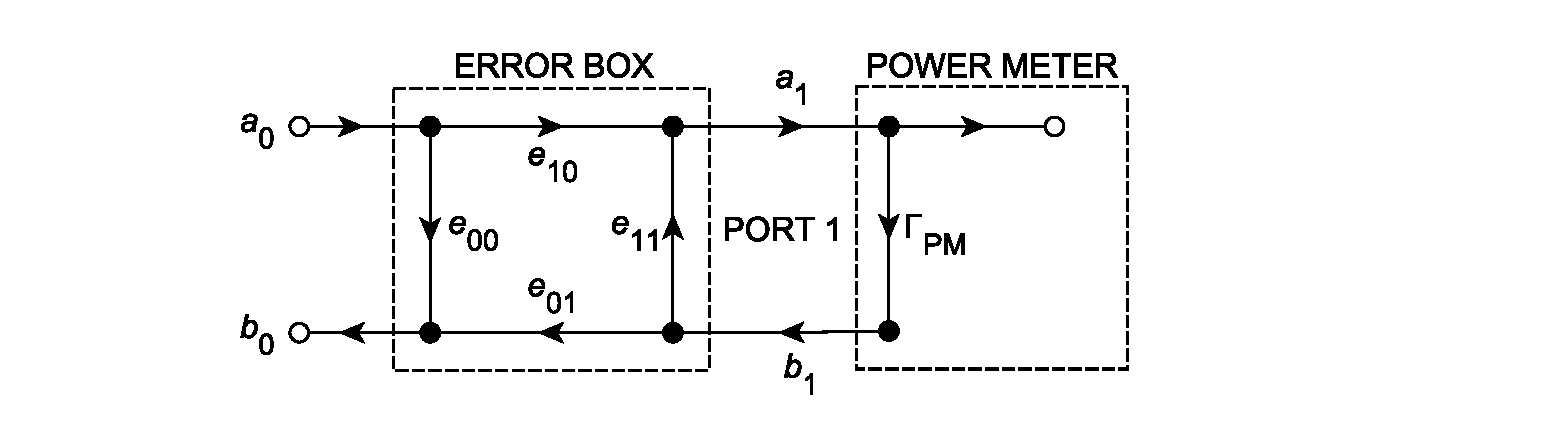
\includegraphics[width=\textwidth]{ch2_powercal}
	\caption[The power calibration of an NVNA.]{Signal flow for the power calibration of an NVNA. The power meter has reflection coefficient $\Gamma_\textrm{PM}$.}
	\label{ch2_fig_powercal}
\end{figure}

\subsection{Phase Reference}

To obtain the phase of $e_{01}$, a phase reference is connected to Port 1 as shown in Figure \ref{ch2_fig_phasecal} and a measurement is made using the test receiver. This equipment produces a frequency comb with highly repeatable and known relative phases, driven from a reference controlled by the NVNA. The comb should contain frequency components (tones) at each of the harmonics which the NVNA is required to measure for the DUTs. More information on the phase reference is given in Chapter 4, Section 5.

The phase of $e_{01}$ can be calculated using:

\begin{align}
	\varphi(e_{01}) &= \varphi\Big(\frac{a_0}{a_\textrm{R}}[\Gamma^\textrm{M}_\textrm{R}-\Gamma^\textrm{M}_\textrm{R}\Gamma_\textrm{R}e_{11}-e_{00}+\Delta\Gamma_\textrm{R}]\Big) \\
	&=\varphi(a_0) + \varphi(\Gamma^\textrm{M}_\textrm{R}-\Gamma^\textrm{M}_\textrm{R}\Gamma_\textrm{R}e_{11}-e_{00}+\Delta\Gamma_\textrm{R}) - \varphi(a_\textrm{R}) \label{ch2_eqn_phasecal}
\end{align}
where $a_\textrm{R}$ is the known signal from the phase reference, $\Gamma^\textrm{M}_\textrm{R}$ is the raw reflection coefficient of the phase reference ($b_0/a_0$) and $\Gamma_\textrm{R}$ is a previously measured and corrected reflection coefficient of the phase reference \cite{Lin_2012}. It can be seen from (\ref{ch2_eqn_phasecal}) that only the phases (relative to the fundamental driving tone) of the phase reference need to be known, and this information is supplied with the equipment.

\begin{figure}
	\centering
	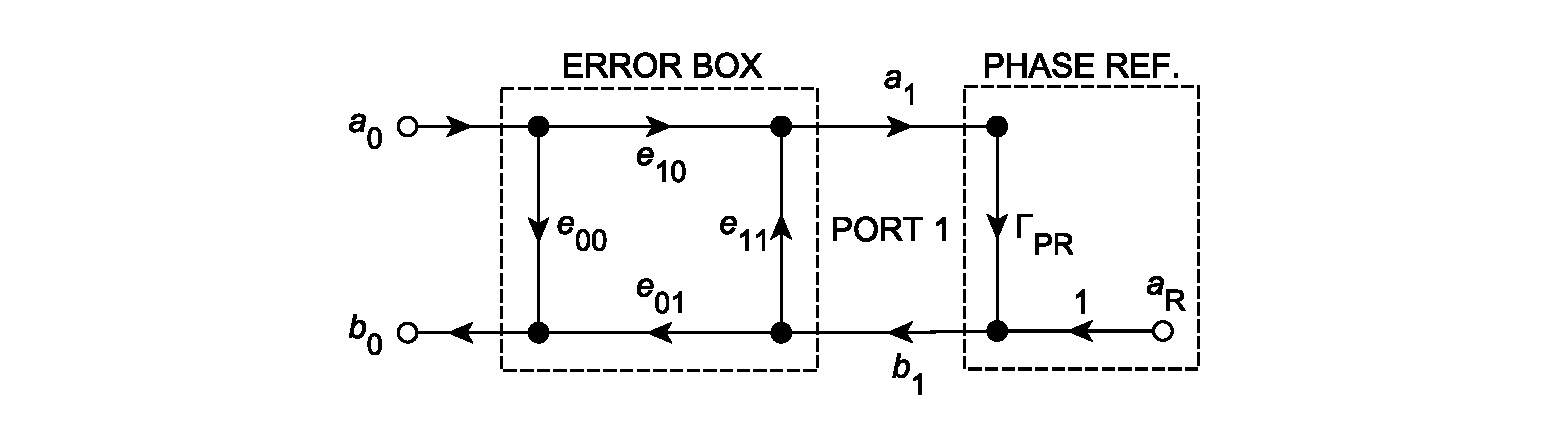
\includegraphics[width=\textwidth]{ch2_phasecal}
	\caption[The phase calibration of an NVNA.]{Signal flow for the phase calibration of an NVNA. The phase reference produces the broadband signal $a_\textrm{R}$ and has reflection coefficient $\Gamma_\textrm{PR}$.}
	\label{ch2_fig_phasecal}
\end{figure}

\section{Conclusions}

This chapter has introduced RF and microwave measurement techniques and given a brief overview of the theory behind VNA and NVNA measurements. Once it was established that electromagnetic wave measurements are not as straightforward as those performed with DC or even low frequency AC circuits, fundamental definitions were presented including the power waves used by VNA and NVNAs. Derived properties such as gain and insertion loss were expressed using S-parameters, which were shown to fully model the frequency-dependent response of a linear $n$-port device. By comparison, the additional measurement challenges required to characterise nonlinear devices could not be contained in the S-parameter model, and more capable solutions are required as covered in Chapter 5.

In the second half of the Chapter, the architecture and operation of the VNA was presented. Calibration models to correct for systematic errors in the instrument and test setup were explained along with the calibration methods used to characterise them. Finally, the NVNA was introduced as an instrument for measuring devices with a nonlinear response, namely microwave power amplifiers. Additional requirements for mixer-based NVNA calibration, in contrast with the VNA it is derived from, were described.

%\addcontentsline{toc}{section}{Bibliography}
%\printbibliography[title=References]
%\end{refsection}
\end{document}
